% Figure 2: validation loss by step.
% source: Hermes report "Validation curve" (HER:137-145); step 300 was measured once in
%   each session, 0.04511 and 0.04512 (plotted 0.04511).
% source: Logos v0.0.1 report "Validation curve" (L1:172-186).
% source: pilot, docs/experiments.md results log (EXP:873-874): 0.03987 at step 200, 0.04469 at step 309.
% source: Logos v0.0.2 report (L2:88): 0.0293 on the loaded best weights (step 175), 0.0311 at step 309.
\begin{figure}[t]
\centering
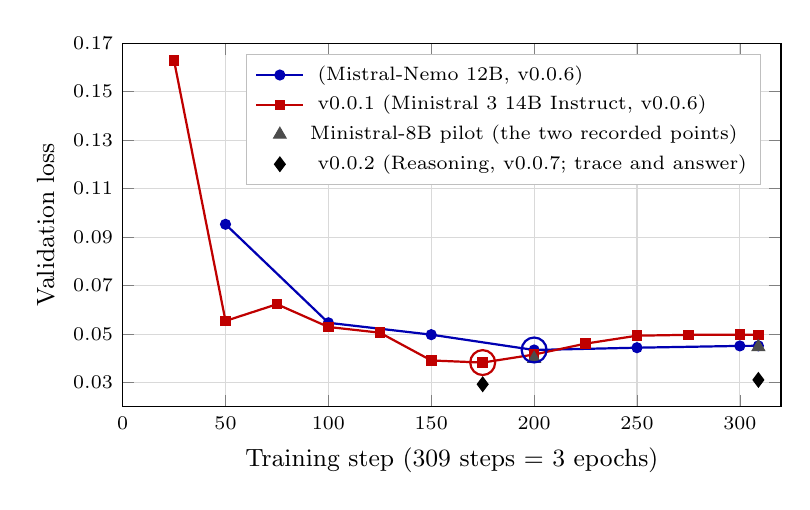
\begin{tikzpicture}
\begin{axis}[
  width=0.82\linewidth, height=6.2cm,
  xlabel={Training step (309 steps $=$ 3 epochs)}, ylabel={Validation loss},
  xmin=0, xmax=320, ymin=0.02, ymax=0.17,
  scaled y ticks=false, yticklabel style={/pgf/number format/fixed, /pgf/number format/precision=2},
  ytick={0.03,0.05,0.07,0.09,0.11,0.13,0.15,0.17},
  grid=major, grid style={gray!30},
  legend pos=north east, legend cell align=left,
  legend style={font=\scriptsize, draw=gray!50},
  tick label style={font=\scriptsize}, label style={font=\small},
]
\addplot[color=blue!70!black, mark=*, mark size=1.6pt, thick] coordinates {
  (50,0.09527) (100,0.05465) (150,0.04975) (200,0.04343) (250,0.04437) (300,0.04511) (309,0.04515)};
\addlegendentry{\hermes{} (Mistral-Nemo 12B, v0.0.6)}
\addplot[color=red!75!black, mark=square*, mark size=1.5pt, thick] coordinates {
  (25,0.16277) (50,0.05541) (75,0.06231) (100,0.05292) (125,0.05057) (150,0.03911) (175,0.03824)
  (200,0.04156) (225,0.04605) (250,0.04933) (275,0.04968) (300,0.04973) (309,0.04969)};
\addlegendentry{\logos{} v0.0.1 (Ministral 3 14B Instruct, v0.0.6)}
\addplot[color=gray!60!black, mark=triangle*, only marks, mark size=2.6pt] coordinates {(200,0.03987) (309,0.04469)};
\addlegendentry{Ministral-8B pilot (the two recorded points)}
\addplot[color=black, mark=diamond*, only marks, mark size=2.6pt] coordinates {(175,0.0293) (309,0.0311)};
\addlegendentry{\logos{} v0.0.2 (Reasoning, v0.0.7; trace and answer)}
\addplot[forget plot, color=blue!70!black, mark=o, only marks, mark size=4.5pt, thick] coordinates {(200,0.04343)};
\addplot[forget plot, color=red!75!black, mark=o, only marks, mark size=4.5pt, thick] coordinates {(175,0.03824)};
\end{axis}
\end{tikzpicture}
\caption{Validation loss by training step. Circles mark the checkpoints that were selected on validation loss and shipped: step 200 (epoch 1.95) for Hermes, 0.04343, and step 175 (epoch 1.70) for Logos v0.0.1, 0.03824. Both recorded curves rise through the third epoch, and in the other two runs the final value exceeds the selected one. The pilot and Logos v0.0.2 records keep only the best and final values; v0.0.2's loss covers the reasoning trace as well as the answer. The tokenizers differ between models, so the curves compare in shape, not in level.}
\label{fig:validation}
\end{figure}
